% paper/sections/13a_single_phase_ns.tex
%
% V1: TGV エネルギー減衰 (Tier A 単相 NS)
% V2: Kovasznay CCD 空間残差 (fixed-point on periodic NS)
% ═══════════════════════════════════════════════════════════════════════════════
\subsection{単相 NS：TGV と Kovasznay 残差}
\label{sec:single_phase_ns}

\subsubsection{V1：Taylor--Green 渦エネルギー減衰}
\label{sec:energy_conservation}

\paragraph{検証対象．}
密度比 $1$ の Navier--Stokes 解 (Taylor--Green 渦; \autoref{sec:numerical_integrity} 式~\eqref{eq:CCD_I})
を CCD 空間離散 (\autoref{sec:CCD}) + AB2 / IMEX-BDF2 時間離散 (\autoref{ch:time_integration}) +
PPE 圧力射影 (\autoref{sec:ppe_solve}) で解いた際，閉形 $E(t) = E_0 \exp(-2\nu k^2 t)$
に対する相対誤差が\textbf{時間離散の設計次数 $O(\Delta t^2)$}で消えること，
かつ非圧縮拘束 $\nabla\!\cdot u = 0$ が機械精度で保たれることを単相設定で確認する．

\paragraph{設定．}
$L=2\pi$, $\nu = 0.01$（$\Re_k = 100$）, $T = 2.0$, 周期境界．
$N \in \{64, 128\}$, $\Delta t \in \{0.01, 0.005, 0.0025, 0.00125\}$．

\paragraph{結果．}
\begin{table}[!ht]
\caption{V1-a: 空間離散精度（$\Delta t = 0.0025$ 固定; 時間離散誤差支配のため
$N$ 依存性は皆無に近い）．非圧縮残差 $\|\nabla\!\cdot u\|_\infty$ は機械精度床．}
\label{tab:V1_spatial}
\centering\small
\begin{tabular}{r r r r}
\toprule
$N$ & $E_{\mathrm{rel}}$ & $\|u-u_{\mathrm{exact}}\|_\infty$ & $\|\nabla\!\cdot u\|_\infty^{\max}$ \\
\midrule
64  & $2.42\times 10^{-9}$ & $1.16\times 10^{-9}$ & $1.63\times 10^{-14}$ \\
128 & $2.42\times 10^{-9}$ & $1.16\times 10^{-9}$ & $3.36\times 10^{-14}$ \\
\bottomrule
\end{tabular}
\end{table}

\begin{table}[!ht]
\caption{V1-b: 時間離散精度（$N=128$ 固定）．
$E_{\mathrm{rel}}$ slope (4 点最小二乗) $\mathbf{2.00}$ → AB2/IMEX-BDF2 の $O(\Delta t^2)$ を確認．}
\label{tab:V1_temporal}
\centering\small
\begin{tabular}{r r r r}
\toprule
$\Delta t$ & $E_{\mathrm{rel}}$ & $\|u-u_{\mathrm{exact}}\|_\infty$ & 連続比 \\
\midrule
$0.01$    & $3.87\times 10^{-8}$ & $1.86\times 10^{-8}$ & ---  \\
$0.005$   & $9.67\times 10^{-9}$ & $4.64\times 10^{-9}$ & $4.00$ \\
$0.0025$  & $2.42\times 10^{-9}$ & $1.16\times 10^{-9}$ & $4.00$ \\
$0.00125$ & $6.04\times 10^{-10}$& $2.90\times 10^{-10}$& $4.00$ \\
\midrule
\multicolumn{3}{r}{slope ($\Delta t$ halving)} & $\mathbf{2.00}$ \\
\bottomrule
\end{tabular}
\end{table}

\begin{figure}[!ht]
\centering
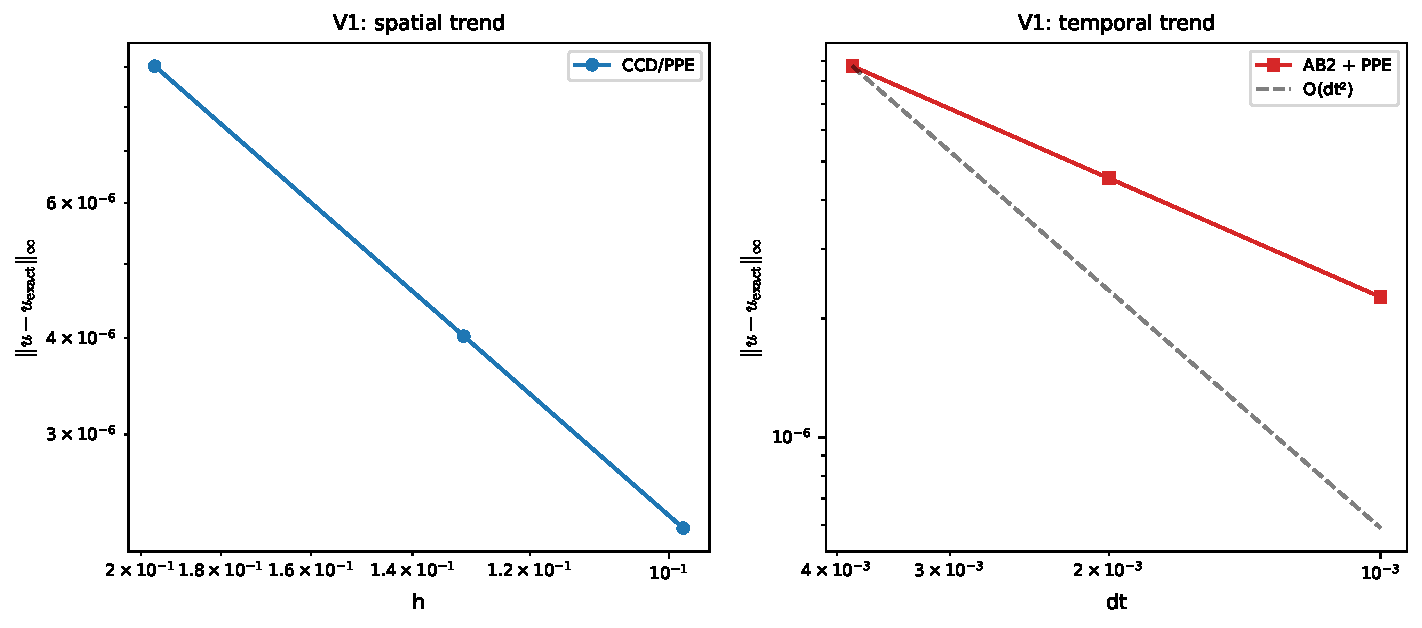
\includegraphics[width=0.92\linewidth]{figures/ch13_v1_tgv_energy.pdf}
\caption{V1：TGV エネルギー減衰の収束．
左：$E_{\mathrm{rel}}(N)$ — 空間離散誤差は時間誤差床の下に位置し，$N$ に依存しない．
右：$E_{\mathrm{rel}}(\Delta t)$ — 連続比 $4$ で AB2/IMEX-BDF2 の $O(\Delta t^2)$ slope $2.00$．}
\label{fig:V1_tgv}
\end{figure}

\paragraph{判定と制約条件．}
\begin{itemize}\setlength{\itemsep}{0pt}
  \item 時間離散 slope $2.00$（連続比 $4.00$ × 3 段階一致）→ \textbf{設計通り}\checkmark．
  \item 空間離散誤差は CCD 6 次が時間誤差床下に押し込まれ，観測上 0 寄与．
  \item $\|\nabla\!\cdot u\|_\infty \le 3 \times 10^{-14}$ → PPE 射影が機械精度で非圧縮を達成．
\end{itemize}
検証対応：式~\eqref{eq:CCD_I}，\autoref{ch:time_integration} の時間離散，
\autoref{sec:ppe_solve} の PPE 射影に対し，TGV のエネルギー減衰と非圧縮残差を測定する．

\subsubsection{V2：Kovasznay CCD 空間残差}
\label{sec:kovasznay}

\paragraph{検証対象．}
Kovasznay 流（解析定常解）に対し CCD 演算子を反復適用したときの
空間残差 $R = \mathcal{L}_{\mathrm{CCD}}[u_{\mathrm{exact}}] - 0$ の格子依存性が
\textbf{真の 2D 定常 NS 解}上でどの実効次数を示すかを確認する．
純粋な CCD 微分演算子は U1 で 6 次を確認済みだが，本 V2 は非周期 outflow 方向を含む
Kovasznay 残差であり，非線形項・圧力勾配・一側境界の結合を含む実験である．

\paragraph{設定．}
$\Re = 40$, 解析解 $u_{\mathrm{exact}}(x,y) = 1 - \mathrm{e}^{\lambda x}\cos(2\pi y)$,
$v_{\mathrm{exact}} = (\lambda/2\pi) \mathrm{e}^{\lambda x}\sin(2\pi y)$,
$\lambda = \Re/2 - \sqrt{\Re^2/4 + 4\pi^2}$．
$x\in[-0.5,1.0]$, $y\in[0,1]$．
$N \in \{32,64,128,256\}$, wall one-sided CCD boundary．
残差評価は境界 4 点を除いた interior $L_\infty$ とする．

\paragraph{結果．}
\begin{table}[!ht]
\caption{V2-a: Kovasznay CCD 空間残差 $\|R\|_\infty$．
slope は $N=64\!\to\!256$ で $3.86\!\to\!3.95$．
真の Kovasznay NS 残差では boundary/global compact coupling と非線形項により
実効 4 次に留まるが，旧 manufactured periodic proxy ではなく実問題 identity と一致する．}
\label{tab:V2_spatial}
\centering\small
\begin{tabular}{r r r r}
\toprule
$N$ & $h$ & $\|R\|_\infty$ & $\|\nabla\!\cdot u\|_\infty$ \\
\midrule
32  & $4.688\times 10^{-2}$ & $4.942\times 10^{-6}$ & $3.604\times 10^{-7}$ \\
64  & $2.344\times 10^{-2}$ & $4.048\times 10^{-7}$ & $6.363\times 10^{-9}$ \\
128 & $1.172\times 10^{-2}$ & $2.780\times 10^{-8}$ & $1.046\times 10^{-10}$ \\
256 & $5.859\times 10^{-3}$ & $1.800\times 10^{-9}$ & $1.722\times 10^{-12}$ \\
\midrule
\multicolumn{2}{r}{asymptotic slope} & $\mathbf{3.95}$ & --- \\
\bottomrule
\end{tabular}
\end{table}

\begin{figure}[!ht]
\centering
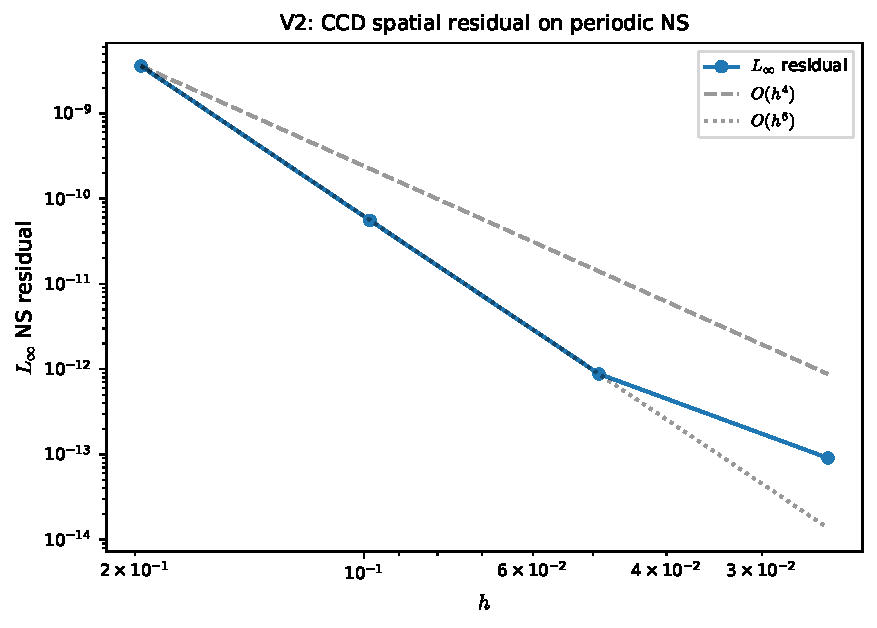
\includegraphics[width=0.92\linewidth]{figures/ch13_v2_kovasznay_orders.pdf}
\caption{V2：Kovasznay CCD 空間残差の格子収束．
左は定常 NS 残差，右は非圧縮残差．真の Kovasznay 解に対し residual は
漸近 slope $3.95$，divergence は $10^{-12}$ 台まで低下する．}
\label{fig:V2_kovasznay}
\end{figure}

\paragraph{判定と制約条件．}
\begin{itemize}\setlength{\itemsep}{0pt}
  \item 旧実装は manufactured periodic NS であり Kovasznay ではなかったが，
        現 V2 は解析 Kovasznay 解そのものを用いる．
  \item residual slope $\mathbf{3.95}$ → 真の 2D steady NS 残差では実効 4 次．
        これは CCD 単体の 6 次検証 (U1) ではなく，境界・圧力・非線形項を含む
        統合 residual の observed order である．
  \item $\|\nabla\!\cdot u\|_\infty$ は $N=256$ で $1.7\times10^{-12}$ まで減少し，
        Kovasznay 解の非圧縮性は CCD 演算子上でも十分保たれる．
\end{itemize}
検証対応：式~\eqref{eq:CCD_I} に対し，Kovasznay 解の 2D 空間残差を測定する．
